\subsection{Database Script}
\begin{figure}[htp]
\centering
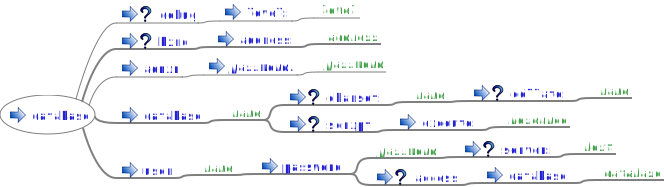
\includegraphics[width=0.9\textwidth]{database_service_script}
\label{fig:database_script_statements}
\caption{Database Script Statements}
\end{figure}


\TheStatement{database}
\TheStatement*[database]{database \{ debugging bind\_address admin\_password database user \}}

Entry point in the database script.

\TheStatement[database:debugging]{debugging}
\TheStatement*[database!debugging]{debugging true|false}

Enables or disables the general logging for the database server.
Default logging is off.

\TheStatement[database:bind_address]{bind\_address}
\TheStatement*[database!bind\_address]{bind\_address \Arg{address}}

The IP \Arg{address} or the host name on which the database server should listen
to connections. Defaults to the localhost address \code{"127.0.0.1"}.

\TheStatement[database:admin_password]{admin\_password}
\TheStatement*[database!admin\_password]{admin\_password \Arg{password}}

The administrator \Arg{password} for the database server. If no password for
the administrator account was yet set this password is set. Used to login as
the administrator user to create users, create databases and set permissions.

\TheStatement[database:db]{database}
\TheStatement*[database!database]{database \Arg{name} [, character\_set: \Arg{name}] [, collate: \Arg{name}] \{ import\_sql \}}

Creates a new database with the specified database \Arg{name}, character set and collate.
If the database was already on the server, it will update the character set and collate
to the specified character set and collate.

The database server needs to support the specified character set and collate.
Defaults to the UTF-8 character set and the UTF-8 general collate:

\begin{compactitem}
\item MySQL: \code{"utf-8"}, \code{"utf8\_general\_ci"}
\end{compactitem}

\TheStatement[database:import_sql]{import\_sql}
\TheStatement*[database!import\_sql]{import\_sql \Arg{resource}}

Imports SQL script \Arg{resource} from the specified file, URL or URI. 
A string will be interpreted according to the format. If no scheme is used 
the string is assumed to be a local file, otherwise the string is assumed to 
be a URI.

\TheStatement[database:user]{user}
\TheStatement*[database!user]{user \Arg{name}, password: \Arg{password} [, server: \Arg{host}] [, \{ use\_database \}]}

Creates a new user with the specified \Arg{name}, \Arg{password} and server \Arg{host}.
If the user already exists on the server, the password is updated for that user.
A user is identified by the user name and the server host.
The server host name defaults to the server host \code{"localhost"}.

The database that the user have read and write access to will be set. This will not create
the database on the server, to create a database use the \TheStatement*{database} statement.
